\section{Zielsetzung}
Ziel des Versuches ist es, die Funktionsweise und das Prinzip der Wärmepumpe durch eine beispielhafte Messung zu zeigen.

\section{Theorie}
\label{sec:Theorie}
Bei der Wärmepumpe handelt es sich um eine Vorrichtung, welche es erlaubt die durch den zweiten Hauptsatz der Thermodynamik gegebene Flussrichtung(vom wärmeren zum kälteren Körper) durch
mechanische Arbeit umzukehren. Die Wärmepumpe ist dabei wie in Abbildung \ref{fig:skizze} dargestellt aufgebaut.
\begin{figure}
  \centering
  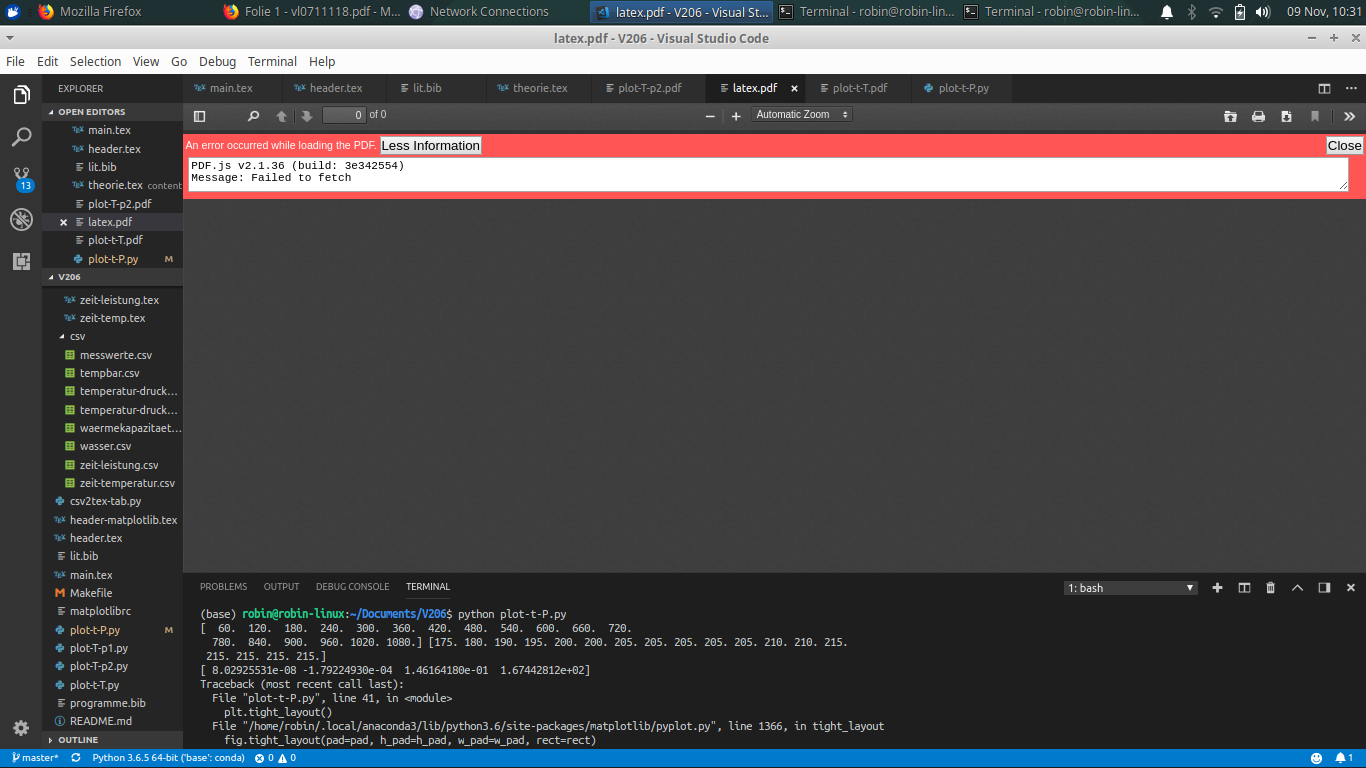
\includegraphics{content/skizze.png}
  \caption{Schematischer Aufbau der Wärmepumpe ***Abbildung noch fehlend*** \cite[193]{206}}
  \label{fig:skizze}
\end{figure}
Der Körper welcher in der Abbildung als Reservoir 1 bezeichnet wird, ist das Objekt, welches beheizt werden soll; das Reservoir 2 liefert die hierzu notwendige Energie.
Wichtig ist, dass es sich bei den Reservoiren um abgeschlossene Systeme handelt, das heißt, dass sie möglichst thermisch isoliert sein müssen.
Durch die beiden Reservoire wird ein reales Gas geleitet, in diesem Fall Dichlordifluormethan, welches die Eigenschaft besitzt den Agregatzustand durch sich verändernden Druck gut wechseln zu können.
Bezogen auf Abbildung \ref{fig:skizze} heißt das, dass das Gas in Reservoir 2 einen Druck $p_2$ und eine Temperatur $T_2$ hat und gasförmig wird, wobei es dem Reservoir 2 die Verdampfungsenergie L entzieht. 
Der Kompressor sorgt dabei für einen Gaskreislauf zwischen den Reservoiren und eine adiabatische Kompression, zwischen den Reservoiren, was heißt, dass dabei keine zusätzliche Wärme an die Umgebung abgegeben wird.
Wenn das gasförmige Gas nun in Reservoir 1 strömt, wird es aufgrund des höheren Druckes $p_1 > p_2$, welcher durch die Kompression vorliegt, wieder flüssig und gibt dabei Wärmeenergie an das Reservoir mit Temperatur $T_1$ ab. Das nun flüssige Gas strömt dann durch ein Drosselventil zurück zu Reservoir 2 und der Kreislauf führt sich fort.
Nach und nach erwärmt sich das Reservoir 1 also, während sich Reservoir 2 nach und nach weiter abkühlt.
In der Praxis können Objekte so durch Reservoire geheizt werden, welche eine nahezu unendliche Menge konstanter Wärmeenergie aufweisen, wie die Umgebungsluft oder das Grundwasser.
Weitere Bauteile neben dem Drosselventil, welches die Menge an einströmden flüssigen Gas reguliert, ein Steuergerät, welches die Regulierung des Drosselventils steuert und ein Reiniger welcher das flüssige Gas von gasförmigen Resten befreit, um den Kompressor zu entlasten.
\subsection{Güteziffer}
\subsection{Massendurchsatz}
\subsection{Mechanische Kompressorleistung}